% !TEX root = saveliev_physics_general_course_2.tex
%!TEX TS-program = pdflatex
%!TEX encoding = UTF-8 Unicode


\chapter[MOTION OF CHARGED PARTICLES IN ELECTRIC\\
AND MAGNETIC FIELDS]{MOTION OF CHARGED \\PARTICLES IN ELECTRIC\\ AND MAGNETIC FIELDS}\label{chap:10}
\chaptermark{MOTION OF CHARGED PARTICLES}

\section{Motion of a Charged Particle in a Homogeneous Magnetic Field}\label{sec:10_1}

Imagine a charge $e'$ moving in a homogeneous magnetic field with the velocity $\vec{v}$ perpendicular to $\vec{B}$.
The magnetic force imparts to the charge an acceleration perpendicular to the velocity
\begin{equation}\label{eq:10_1}
    \ab{a}{n} = \frac{F}{m} = \frac{e'}{m} vB
\end{equation}

\noindent
[see \eqn{6_33}; the angle between $\vec{v}$ and $\vec{B}$ is a right one].
This acceleration changes only the direction of the velocity, while the magnitude of the latter remains unchanged.
Hence, the acceleration given by \eqn{10_1} will be constant in magnitude too.
In these conditions, the charged particle moves uniformly around a circle whose radius is determined by means of the equation $\ab{a}{n}=v^2/R$.
Substituting for $\ab{a}{n}$ in this equation its value from \eqn{10_1} and solving the resulting equation relative to $R$, we get
\begin{equation}\label{eq:10_2}
    R = \frac{m}{e'} \frac{v}{B}.
\end{equation}

Thus, when a charged particle moves in a homogeneous magnetic field perpendicular to the plane in which the motion is taking place, the trajectory of the particle is a circle.
The radius of the circle depends on the velocity of the particle, the magnetic induction of the field, and the ratio of the charge of the particle $e'$ to its mass $m$.
The ratio $e'/m$ is called the \textbf{specific charge}.

Let us find the time $T$ needed for the particle to complete one revolution.
For this purpose, we shall divide the length of the circumference $2\pi R$ by the velocity of the particle $v$. The result is
\begin{equation}\label{eq:10_3}
    T = 2\pi \frac{m}{e'} \frac{1}{B}.
\end{equation}

\noindent
Inspection of \eqn{10_3} shows that the period of revolution of the particle does not depend on its velocity.
It is determined only by the specific charge of the particle and the magnetic induction of the field.

Let us determine the nature of motion of a charged particle when its velocity makes the angle $\alpha$ with the direction of a homogeneous magnetic field, and $\alpha$ is not a right angle.
We shall resolve the vector $\vec{v}$ into two components: $\vec{v}_{\perp}$ perpendicular to $\vec{B}$, and $\vec{v}_{\parallel}$ parallel to $\vec{B}$ (\fig{10_1}).
The magnitudes of these components are
\begin{equation*}
    v_{\perp} = v\sin\alpha,\quad v_{\parallel}=v\cos\alpha.
\end{equation*}

The magnetic force has the magnitude
\begin{equation*}
    F = e' v B \sin\alpha = e' v_{\perp} B,
\end{equation*}

\noindent
and is in a plane at right angles to $\vec{B}$.
The acceleration produced by this force is normal for the component $\vec{v}_{\perp}$.
The component of the magnetic force in the direction of $\vec{B}$ is zero.
Hence, this force cannot affect the magnitude of $\vec{v}_{\parallel}$.
The motion of the particle can, thus, be considered as the superposition of two motions: (1) translation along the direction of $\vec{B}$ with a constant velocity $v_{\parallel}=v\cos\alpha$, and (2) uniform circular motion in a plane at right angles to the vector $\vec{B}$.

\begin{figure}[t]
	\begin{minipage}[t]{0.48\linewidth}
		\begin{center}
			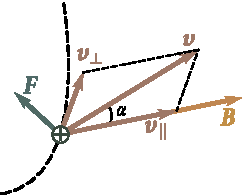
\includegraphics[scale=1]{figures/ch_10/fig_10_1.pdf}
			\caption[]{}
			\label{fig:10_1}
		\end{center}
	\end{minipage}
	\hfill{ }%space{-0.05cm}
	\begin{minipage}[t]{0.48\linewidth}
		\begin{center}
			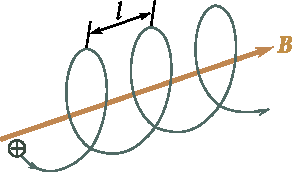
\includegraphics[scale=1]{figures/ch_10/fig_10_2.pdf}
			\caption[]{}
			\label{fig:10_2}
		\end{center}
	\end{minipage}
\vspace{-0.4cm}
\end{figure}

The radius of the circle is determined by \eqn{10_2} with $v_{\perp} = v\sin\alpha$ substituted for $v$.
The trajectory of motion is a helix (spiral) whose axis coincides with the direction of $\vec{B}$ (\fig{10_2}).
The pitch of the helix $l$ can be found by multiplying $v_{\parallel}$ by the period of revolution $T$ determined by \eqn{10_3}:
\begin{equation}\label{eq:10_4}
    l = v_{\parallel} T = 2\pi \frac{m}{e'} \frac{1}{B} v \cos\alpha.
\end{equation}

The direction in which the helix curls depends on the sign of the particle's charge.
If the latter is positive, the helix curls counterclockwise.
A helix along which a negatively charged particle is moving curls clockwise (it is assumed that we are looking at the helix along the direction of $\vec{B}$; the particle flies away from us if $\alpha<\pi/2$, and toward us if $\alpha>\pi/2$).

\section{Deflection of Moving Charged Particles
by an Electric and a Magnetic Field}\label{sec:10_2}

Let us consider a narrow beam of identically charged particles (for example, electrons) that in the absence of fields falls on a screen perpendicular to it at point $0$ (\fig{10_3}).
Let us find the displacement of the trace of the beam produced by a homogeneous electric field perpendicular to the beam and acting on a path of length $l_1$.
Let the initial velocity of the particles be $\vec{v}_0$.
Upon entering the region of the field, each particle will move with an acceleration $a_{\perp}=(e'/m)E$ constant in magnitude and in direction and perpendicular to $\vec{v}_0$ (here, $e'/m$ is the specific charge of a particle).
Motion under the action of the field continues during the time $t = l_1/v_0$.
During this time, the particles will be displaced over the distance
\begin{equation}\label{eq:10_5}
    y_1 = \frac{1}{2} a_{\perp} t^2 = \frac{1}{2} \frac{e'}{m} E \frac{l_1^2}{v_0^2},
\end{equation}

\noindent
and will acquire the following velocity component perpendicular to $\vec{v}_0$:
\begin{equation*}
    v_{\perp} = a_{\perp} t = \frac{e'}{m} E \frac{l_1}{v_0}.
\end{equation*}

\begin{figure}[t]
	\begin{center}
		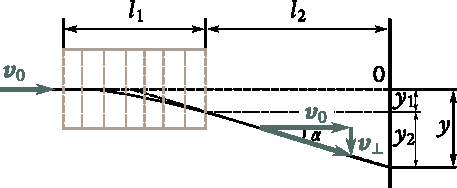
\includegraphics[scale=0.98]{figures/ch_10/fig_10_3.pdf}
		\caption[]{}
		\label{fig:10_3}
	\end{center}
	\vspace{-0.85cm}
\end{figure}

The particles now fly in a straight line in a direction that makes with the vector $\vec{v}_0$ the angle $\alpha$ determined by the expression
\begin{equation}\label{eq:10_6}
    \tan\alpha = \frac{v_{\perp}}{v_0} - \frac{e'}{m} E \frac{l_1}{v_0^2}.
\end{equation}

\noindent
As a result in addition to the displacement given by \eqn{10_5} the beam receives the displacement
\begin{equation*}
    y_2 = l_2 \tan\alpha = \frac{e'}{m} E \frac{l_1 l_2}{v_0^2},
\end{equation*}

\noindent
where $l_2$ is the distance to the screen from the boundary of the region which the field is in.

The displacement of the trace of the beam relative to point $0$ is thus
\begin{equation}\label{eq:10_7}
    y = y_1 + y_2 = \frac{e'}{m} E \frac{l_1}{v_0^2} \parenthesis{\frac{1}{2} l_1 + l_2}.
\end{equation}

\noindent
Taking into account \eqn{10_6}, the expression for the displacement can be written in the form
\begin{equation*}
    y = \parenthesis{\frac{1}{2} l_1 + l_2} \tan\alpha.
\end{equation*}

\noindent
It thus follows that the particles leaving the field fly as if they were leaving the centre of the capacitor setting up the field at the angle $\alpha$ determined by means of \eqn{10_6}.

Now let us assume that on a particle path of $l_1$ a homogeneous magnetic field is switched on perpendicular to the velocity $\vec{v}_0$ of the particles (\fig{10_4}; the field is perpendicular to the plane of the drawing, the region of the field is surrounded by a dash circle).
Under the action of the field, each particle receives the acceleration $a_{\perp}=(e'/m)v_0B$ constant in magnitude.
Limiting ourselves to the case when the deflection of the beam by the field is not great, we can consider that the acceleration $a_{\perp}$ is constant in magnitude and perpendicular to $v_0$.
Hence, we can use the equations we have obtained for calculating the displacement, replacing the acceleration $a_{\perp}=(e'/m)E$ in them with the value $a_{\perp}=(e'/m)v_0B$.
As a result, we get the following expression for the displacement, which we shall now denote by $x$:
\begin{equation}\label{eq:10_8}
    x = \frac{e'}{m} B \frac{l_1}{v_0} \parenthesis{\frac{1}{2} l_1 + l_2}.
\end{equation}

\begin{figure}[t]
	\begin{center}
		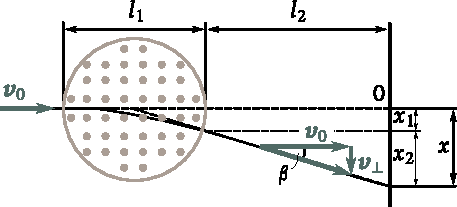
\includegraphics[scale=0.98]{figures/ch_10/fig_10_4.pdf}
		\caption[]{}
		\label{fig:10_4}
	\end{center}
	\vspace{-0.85cm}
\end{figure}

The angle through which the beam is deflected by the magnetic field is determined by the expression
\begin{equation}\label{eq:10_9}
    \tan\beta = \frac{e'}{m} B \frac{l_1}{v_0}.
\end{equation}

\noindent
With a view to \eqn{10_3}, we can write \eqn{10_8} in the form
\begin{equation*}
    x = \parenthesis{\frac{1}{2} l_1 + l_2} \tan\beta.
\end{equation*}

\noindent
Consequently, upon small deflections, the particles after leaving the magnetic field fly as if they had left the centre of the region containing the deflecting field at the angle $\beta$ whose magnitude is determined by \eqn{10_9}.

Inspection of \eqns{10_7}{10_8} shows that both the deflection by an electric field and the deflection by a magnetic one are proportional to the specific charge of the particles.

The deflection of a beam of electrons by an electric or magnetic field is used in cathode-ray tubes.
A tube with electrical deflection (\fig{10_5}), apart from the so-called electron gun producing a narrow beam of fast electrons (an electron beam), contains two pairs of mutually perpendicular deflecting plates.
By feeding a voltage to any pair of plates, we can produce a proportional displacement of the electron beam in a direction normal to the given plates.
The screen of the tube is coated with a fluorescent composition.
Therefore, a brightly luminescent spot appears on the screen where the electron beam falls on it.

\begin{figure}[t]
	\begin{center}
		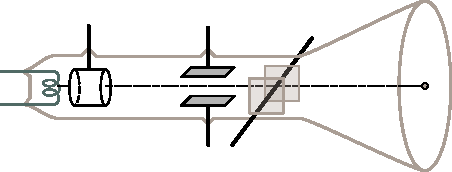
\includegraphics[scale=1]{figures/ch_10/fig_10_5.pdf}
		\caption[]{}
		\label{fig:10_5}
	\end{center}
	\vspace{-0.8cm}
\end{figure}

Cathode-ray tubes are used in oscillographs---instruments making it possible to study rapid processes.
A voltage changing linearly with time (the scanning voltage) is fed to one pair of deflecting plates, and the voltage being studied to the other.
Owing to the negligibly small inertia of an electron beam, its deflection without virtually any delay follows the changes in the voltages across both pairs of deflecting plates, and the beam draws on the oscillograph screen a plot of time dependence of the voltage being studied.
Many nonelectrical quantities can be transformed into electric voltages with the aid of the relevant devices (transducers).
Consequently, oscillographs are used to study the most diverse processes.

A cathode-ray tube is an integral part of television equipment.
In television, tubes with magnetic control of the electron beam are used most frequently.
In these tubes, the deflecting plates are replaced with two external mutually perpendicular systems of coils each of which sets up a magnetic field perpendicular to the beam.
Changing of the current in the coils produces motion of the light spot created by the electron beam on the screen.

\section{Determination of the Charge and Mass
of an Electron}\label{sec:10_3}

The specific charge of an electron (\ie, the ratio $e/m$) was first measured by the British physicist Joseph J. Thomson (1856-1940) in i897 with the aid of a discharge tube like the one shown in \fig{10_6}.
The electron beam (cathode rays; see \sect{12_6}) emerging from the opening in anode A passed between the plates of a parallel-plate capacitor and impinged on a fluorescent screen producing a light spot on it.
By feeding a voltage to the capacitor plates, it was possible to act on the beam with a virtually homogeneous electric field.

\begin{figure}[t]
	\begin{center}
		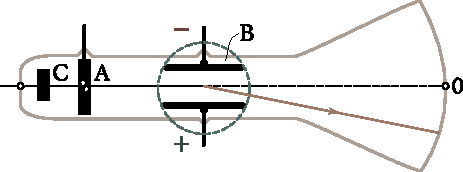
\includegraphics[scale=1]{figures/ch_10/fig_10_6.pdf}
		\caption[]{}
		\label{fig:10_6}
	\end{center}
	\vspace{-0.8cm}
\end{figure}

The tube was placed between the poles of an electromagnet, which could produce a homogeneous magnetic field perpendicular to the electric one on the same portion of the path of the electrons (the region of the magnetic field is shown in \fig{10_6} by the dash circle).
When the fields were switched off, the beam impinged on the screen at point $0$.
Each of the fields separately caused deflection of the beam in a vertical direction.
The magnitudes of the displacements were determined with the aid of \eqns{10_7}{10_8} obtained in the
preceding section.

After switching on the magnetic field and measuring the displacement of the beam trace
\begin{equation}\label{eq:10_10}
    x = \frac{e}{m} B \frac{l_1}{v_0} \parenthesis{\frac{1}{2} l_1 + l_2},
\end{equation}

\noindent
which it produced, Thomson also switched on the electric field and selected its value so that the beam would again reach point $0$.
In this case, the electric and magnetic fields acted on the electrons of the beam simultaneously with forces identical in value, but opposite in direction.
The condition was observed that
\begin{equation}\label{eq:10_11}
    eE = ev_0 B.
\end{equation}

\noindent
By solving the simultaneous equations \eqref{eq:10_10} and \eqref{eq:10_11}, Thomson
calculated $e/m$ and $v_0$.
H. Busch used the method of magnetic focussing to determine the specific charge of electrons.
The essence of this method consists in the following.
Assume that a slightly diverging beam of electrons having a velocity $v$ identical in magnitude flies out from a certain point of a homogeneous magnetic field.
The beam is symmetrical relative to the direction of the field.
The directions in which the electrons fly out form small angles $\alpha$ with the direction of $\vec{B}$.
It was shown in \sect{10_1} that the electrons in this case travel along helical trajectories, performing during the identical time
\begin{equation*}
    T = 2\pi \frac{m}{e} \frac{1}{B},
\end{equation*}

\noindent
a complete revolution and being displaced along the direction of the field over the distance $l$ equal to
\begin{equation}\label{eq:10_12}
    l = v\cos\alpha \times T.
\end{equation}

\noindent
Owing to the smallness of the angles $\alpha$, the distances \eqref{eq:10_12} for different electrons are virtually the same and equal $vT$ (for small angles $\cos\alpha\approx 1$).
Consequently, the slightly diverging beam is focussed at a point that is at the distance
\begin{equation}\label{eq:10_13}
    l = vT = 2 \pi \frac{m}{e} \frac{v}{B}
\end{equation}

\noindent
from the point of emergence of the electrons.

\begin{figure}[t]
	\begin{center}
		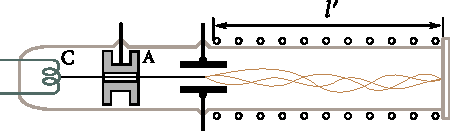
\includegraphics[scale=1]{figures/ch_10/fig_10_7.pdf}
		\caption[]{}
		\label{fig:10_7}
	\end{center}
	\vspace{-0.8cm}
\end{figure}

In Busch's experiment, the electrons emitted by hot cathode C (\fig{10_7}) are accelerated when passing through the potential difference $U$ applied between the cathode and anode A.
As a result, they acquire the velocity $v$ whose value can be found from the relation
\begin{equation}\label{eq:10_14}
    eU = \frac{mv^2}{2}.
\end{equation}

\noindent
After next flying out through an opening in the anode, the electrons form a narrow beam directed along the axis of the evacuated tube inserted into a solenoid.
A capacitor fed with a varying voltage is placed at the inlet of the solenoid.
The field set up by the capacitor deflects the electrons of the beam from the axis of the instrument
through small angles $\alpha$ changing with time.
This leads to ``eddying'' of the beam---the electrons begin to move along different helical trajectories.
A fluorescent screen is placed at the outlet from the solenoid.
If the magnetic induction $B$ is selected so that the distance $l'$ from the capacitor to the screen complies with the condition
\begin{equation}\label{eq:10_15}
    l' = n l
\end{equation}

\noindent
($l$ is the pitch of the helix, and $n$ is an integer), then the point of intersection of the trajectories of the electrons gets onto the screen the electron beam is focussed at this point and produces a sharp luminescent spot on the screen.
If condition \eqref{eq:10_15} is not observed, the luminescent spot on the screen will be blurred.
We can find $e/m$ and $v$ by solving the system of equations \eqref{eq:10_13}, \eqref{eq:10_14}, and
\eqref{eq:10_15}.

The most accurate value of the specific charge of an electron established with account taken of the results obtained by different methods, is
\begin{equation}\label{eq:10_16}
    \frac{e}{m} = \SI{1.76e11}{\coulomb\per\kilo\gram} = \num{5.27e17} \cgs{e}{q}\,\si{\per\gram}.
\end{equation}

\begin{figure}[t]
	\begin{center}
		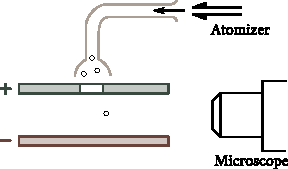
\includegraphics[scale=1]{figures/ch_10/fig_10_8.pdf}
		\caption[]{}
		\label{fig:10_8}
	\end{center}
	\vspace{-0.8cm}
\end{figure}

Equation \eqref{eq:10_16} gives the ratio of the charge of an electron to its rest mass $m$.
In the experiments conducted by Thomson, Busch, and in other similar experiments, the ratio of the charge to the relativistic mass
\begin{equation}\label{eq:10_17}
    \ab{m}{r} = \frac{m}{\sqrt{1 - \parenthesis{v^2/c^2}}},
\end{equation}

\noindent
was determined.
In Thomson's experiments, the speed of the electrons was about $0.1c$.
At such a speed, the relativistic mass exceeds the rest mass by $0.5\%$.
In subsequent experiments, the speed of the electrons reached very high values.
In all cases, the experimenters discovered a reduction in the measured values of $e/m$ with a growth in $v$, which occurred in complete accordance with \eqn{10_17}.

The charge of an electron was determined with high accuracy by the American scientist Robert Millikan (1886-1953) in 1909.
He introduced very minute oil droplets into the closed space between horizontally arranged capacitor plates (\fig{10_8}).
When atomized, the droplets became electrolyzed, and they could be suspended in mid air by properly choosing the magnitude and the sign of the voltage across the capacitor.
Equilibrium set in when the following condition was observed:
\begin{equation}\label{eq:10_18}
    P' = e' E.
\end{equation}

\noindent
Here, $e'$ is the charge of a droplet, and $P'$ is the resultant of the force of gravity and the buoyant force equal to
\begin{equation}\label{eq:10_19}
    P' = \frac{4}{3} \pi r^2 (\rho - \rho_0) g
\end{equation}

\noindent
($\rho$ is the density of a droplet, $r$ is its radius, and $\rho_0$ is the density of air).

Equations \eqref{eq:10_18} and \eqref{eq:10_19} can be used to find $e$ if we know $r$.
To determine the radius, the speed $v_0$ of uniform falling of a droplet was measured in the absence of a field.
Uniform motion of a droplet sets in provided that the force $P'$ is balanced by the force of resistance $F = 6\pi\eta rv$ [see Eq. (9.24) of Vol. I; $\eta$ is the viscosity of air]:
\begin{equation}\label{eq:10_20}
    P' = 6 \pi \eta r v_0.
\end{equation}

\noindent
The motion of a droplet was observed with the aid of a microscope.
To measure $v_0$, the time was determined during which a droplet covered the distance between two threads that could be seen in the field of vision of the microscope.

It is very difficult to accurately suspend a droplet in equilibrium.
Therefore, instead of a field complying with condition \eqref{eq:10_18}, such a field was switched on under whose action a droplet began to move upward with a small speed.
The steady speed of rising $v_E$ is determined from the condition that the force $P'$ and the force $6\pi\eta rv$ together balance the force $e'E$:
\begin{equation}\label{eq:10_21}
    P' + 6\pi\eta rv_E = e'E.
\end{equation}

Excluding $P'$ and $r$ from Eqs. \eqref{eq:10_19}, \eqref{eq:10_20}, and \eqref{eq:10_21}, we get an expression for $e'$:
\begin{equation}\label{eq:10_22}
    e' = 9\pi \bracket{ \frac{2\eta^3 v_0}{(\rho-\rho_0)g} }^{1/2} \parenthesis{ \frac{v_0+v_E}{E} }
\end{equation}

\noindent
(Millikan introduced a correction into this equation taking into account that the dimensions of the droplets were comparable with the free path of air molecules).

Thus, by measuring the speed of free fall of a droplet $v_0$ and the speed of its rise $v_E$ in a known electric field $E$, one could find the charge of a droplet $e'$.
In measuring the speed $v_E$ at a certain value of the charge $e'$, Millikan ionized the air by radiating X-rays through the space between the plates.
Separate ions adhered to a droplet and changed its charge.
As a result, the speed $v_E$ also changed.
After measuring the new value of the speed, the space between the plates was again irradiated, and so on.

The changes in the charge of a droplet $\Delta{e'}$ and the charge $e'$ itself measured by Millikan were each time found to be integral multiples of the same quantity $e$.
This was an experimental proof of the discrete nature of an electric charge, \ie, of the fact that any charge consists of elementary charges of the same magnitude.

The value of the elementary charge established with a view to Millikan's measurements and to the data obtained in other ways is
\begin{equation}\label{eq:10_23}
    e = \SI{1.60e-19}{\coulomb} = \SI{4.80e-10} {\cgs{e}{q}}.
\end{equation}

\noindent
The charge of an electron has the same value.

The rest mass of an electron obtained from \eqns{10_16}{10_23} is
\begin{equation}\label{eq:10_24}
    m = \SI{0.91e-30}{\kilo\gram} = \SI{0.91e-23} {\gram}.
\end{equation}

\noindent
It is about $1/1840$ of the mass of the lightest of all atoms-the hydrogen atom.

The laws of electrolysis established experimentally by Michael Faraday in 1836 played a great part in discovering the discrete nature of electricity.
According to these laws, the mass $m$ of a substance
liberated when a current passes through an electrolyte\footnote{Electrolytes are solutions of salts, alkalies or acids in water and some other
liquids, and also molten salts that are ionic crystals in the solid state. Chemical transformations occur in electrolytes when a current passes through them. Such substances are called electrolytic conductors (conductors of the second kind) to distinguish them from electronic conductors (conductors of the first kind) in which the passage of a current is not attended by chemical transformations.} is proportional to the charge $q$ carried by the current:
\begin{equation}\label{eq:10_25}
    m = \frac{1}{F} \frac{M}{z} q.
\end{equation}

\noindent
Here, $M$ is the mass of one mole of the liberated substance, $z$ the valence of the substance and $F$ the \textbf{Faraday's constant} (\textbf{Faraday's number}) equal to
\begin{equation}\label{eq:10_26}
    F = \SI{96.5e3}{\coulomb\per\mole}.
\end{equation}

Dividing both sides of \eqn{10_25} by the mass of an ion, we get
\begin{equation*}
    N = \frac{1}{F} \frac{\ab{N}{A}}{z} q,
\end{equation*}

\noindent
where $\ab{N}{A}$ is the Avogadro's constant and $N$ the number of ions contained in the mass $m$.

Hence, for the charge of one ion, we have
\begin{equation*}
    e' = \frac{q}{N} = \frac{F}{\ab{N}{A}} z.
\end{equation*}

\noindent
Consequently, the charge of an ion is an integral multiple of the quantity
\begin{equation}\label{eq:10_27}
    e = \frac{F}{\ab{N}{A}},
\end{equation}

\noindent
which is the elementary charge.

Thus, the discrete nature of the charges which ions in electrolytes can have follows from an analysis of the laws of electrolysis.

Substituting for $F$ in \eqn{10_27} its value from \eqn{10_26} and for $\ab{N}{A}$ its value found from J. Perrin's experiments (see Sec. 11.9 of Vol. I), we get a value fore that agrees quite well with that
found by Millikan.

Since the accuracy with which Faraday's constant is determined and the accuracy of the value of $e$ obtained by Millikan are greatly superior to the accuracy of Perrin's experiments for determining $\ab{N}{A}$, \eqn{10_27} was used to determine Avogadro's constant.
Here, the value of $F$ found from experiments in electrolysis and the value of $e$ obtained by Millikan were used.

\section{Determination of the Specific Charge of Ions. Mass Spectrographs}\label{sec:10_4}

The methods of determining the specific charge described in the preceding section are suitable when all the particles in a beam have the same velocity.
All the electrons forming a beam are accelerated by the same potential difference applied between the cathode from which they fly out and the anode.
Therefore, the scattering of the values of the velocities of the electrons in a beam is very small.
If matters were different, an electron beam would produce a greatly blurred spot on the screen, and measurements would be impossible.

Ions are formed as a result of ionization of molecules of a gas that takes place in a volume having an appreciable length.
Appearing in different places of this volume, the
ions then pass through different potential differences, and, consequently, their velocities are different.
Thus, the methods used to determine the specific charge of electrons cannot be applied to ions.
In 1907, J. J. Thomson developed the ``method of parabolas'', which made it possible to circumvent the
difficulty noted above.

\begin{figure}[t]
	\begin{center}
		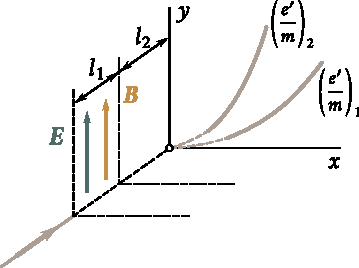
\includegraphics[scale=1]{figures/ch_10/fig_10_9.pdf}
		\caption[]{}
		\label{fig:10_9}
	\end{center}
	\vspace{-0.8cm}
\end{figure}

In Thomson's experiment, a narrow beam of positive ions passed through a region in which it simultaneously experienced the action of parallel electric and magnetic fields (\fig{10_9}).
Both fields were virtually homogeneous and made a right angle with the initial direction of the beam.
They produced deflections of the ions: the magnetic
field deflected them in the direction of the $x$-axis, the electric one along they $y$-axis.
According to \eqns{10_8}{10_7}, these deflections
are
\begin{equation}\label{eq:10_28}
    \begin{split}
        x &= \frac{e'}{m} B \frac{l_1}{v} \parenthesis{\frac{1}{2} l_1 + l_2}\\
        y &= \frac{e'}{m} E \frac{l_1}{v^2} \parenthesis{\frac{1}{2} l_1 + l_2},
    \end{split}
\end{equation}

\noindent
where $v$ is the velocity of a given ion with the specific charge $e'/m$, $l_1$ the length of the region in which the field acts on the beam and $l_2$ is the distance from the boundary of this region to the photographic plate registering the ions impinging on it.

Equations \eqref{eq:10_28} are the coordinates of the point at which an ion having the given values of $e'/m$ and the velocity $v$ impinges on the plate.
Ions having the same specific charge, but different velocities, reached different points of the plate.
Eliminating the velocity $v$ from Eqs. \eqref{eq:10_28}, we get the equation of a curve along which the traces of ions having the same value of $e'/m$ are arranged:
\begin{equation}\label{eq:10_29}
    y = \frac{E}{B^2 l_1 (0.5 l_1 + l_2)} \frac{m}{e'} x^2.
\end{equation}

Inspection of \eqn{10_29} shows that ions having identical values of $e'/m$ and different values of $v$ left a trace in the form of a parabola on the plate.
Ions having different values of $e'/m$ occupied different parabolas.
Equation \eqref{eq:10_29} can be used to find the specific charge of the ions corresponding to each parabola if the parameters of the instrument are known (\ie, $E$, $B$, $l_1$, and $l_2$), and the displacements $x$ and $y$ are measured.
When the direction of one of the fields was reversed, the relevant coordinate reversed its sign, and parabolas symmetrical to the initial ones were obtained.
Dividing the distance between similar points of symmetrical parabolas in half made it possible to find $x$ and $y$.
The trace left on the plate by the beam with the fields switched off gave the origin of coordinates. Figure \ref{fig:10_10} shows the first parabolas obtained by Thomson.

\begin{figure}[t]
	\begin{center}
		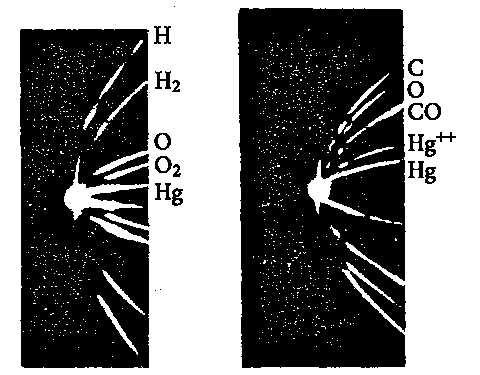
\includegraphics[scale=0.9]{figures/ch_10/fig_10_10.pdf}
		\caption[]{}
		\label{fig:10_10}
	\end{center}
	\vspace{-0.8cm}
\end{figure}

When performing experiments with chemically pure neon, Thomson discovered that this gas produced two parabolas corresponding to relative atomic masses of $20$ and $22$.
This result gave rise to the assumption that there are two chemically indistinguishable varieties of the neon atoms (today we call them \textbf{isotopes} of neon).
This assumption was proved by the British scientist Francis Aston (1877-1945), who improved the method of determining the specific charge of ions.

\begin{figure}[t]
	\begin{center}
		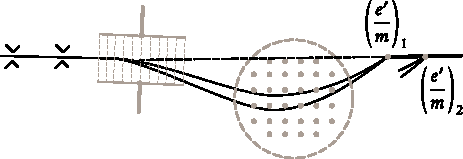
\includegraphics[scale=1]{figures/ch_10/fig_10_11.pdf}
		\caption[]{}
		\label{fig:10_11}
	\end{center}
	\vspace{-0.75cm}
\end{figure}

Aston's instrument, which he called a \textbf{mass spectrograph}, was designed as follows (\fig{10_11}).
A beam of ions separated by a system of slits was consecutively passed through an electric field and a magnetic field.
These fields were directed so that they caused the ions to travel to opposite sides.
When they passed through the electric field, ions with a given value of $e'/m$ were deflected more when their velocity was lower.
Consequently, the ions left the electric field in the form of a diverging beam.
The trajectories of the ions were also curved more in the magnetic field when their velocity was lower.
Since the ions were deflected to opposite sides by the two fields, after leaving the magnetic field they formed a beam converging at one point.

\begin{figure}[t]
	\begin{center}
		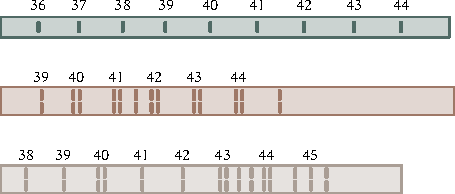
\includegraphics[scale=0.93]{figures/ch_10/fig_10_12.pdf}
		\caption[]{}
		\label{fig:10_12}
	\end{center}
	\vspace{-0.9cm}
\end{figure}

Ions with other values of the specific charge were focussed at other points (the trajectories of the ions for only one value of $e'/m$ are shown in \fig{10_11}).
The relevant calculations show that points at which beams formed by ions having different values of $e'/m$ converge are approximately on a single straight line (shown by a dash line in the figure).
Putting a photographic plate along this line, Aston obtained a number of short lines on it, each of which corresponded to a definite value of $e'/m$.
The similarity of the image obtained on the plate to a photograph of an optical line spectrum was the reason why Aston called it a mass spectrogram, and the instrument itself---a mass spectrograph.
Figure \ref{fig:10_12} shows mass spectrograms obtained by Aston (the mass numbers of the relevant ions are indicated opposite the lines).

K. Bainbridge designed an instrument of a different kind.
In the Bainbridge mass spectrograph (\fig{10_13}), a beam of ions first passes through the so-called velocity selector that separates ions having a definite velocity from the beam.
In the selector, the ions experience the action of mutually perpendicular electric and magnetic fields that deflect the ions to opposite sides.
Only those ions pass through the selector slit for which the actions of the electric and magnetic fields compensate each other.
This occurs when $e'E = e'vB$.
Hence, the velocities of the ions leaving the selector regardless of their mass and charge have identical values equal to $v = E/B$.

\begin{figure}[t]
	\begin{center}
		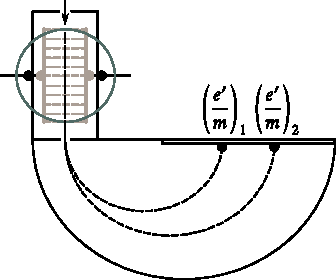
\includegraphics[scale=1]{figures/ch_10/fig_10_13.pdf}
		\caption[]{}
		\label{fig:10_13}
	\end{center}
	\vspace{-0.8cm}
\end{figure}

After leaving the selector, the ions get into the region of a homogeneous magnetic field of induction $B'$ at right angles to their velocity.
In this field, they move along circles whose radii depend on $e'/m$:
\begin{equation*}
    R = \frac{m}{e'}\frac{v}{B'}
\end{equation*}

[see \eqn{10_21}].

After completing a semi-circle, the ions strike a photographic plate at distances of $2R$ from the slit.
Hence, the ions of each species (determined by the value of $e'/m$) leave a trace on the plate in the form of a narrow strip.
The specific charges of the ions can be calculated if the parameters of the instrument are known.
Since the charges of the ions are integral multiples of the elementary charge $e$, the masses of the ions can be calculated from the found values of $e'/m$.

Numerous kinds of mass spectrographs are in use at present.
Instruments have also been designed in which the ions are registered by means of an electrical device instead of by a photographic plate.
They are called \textbf{mass spectrometers}.

\section{Charged Particle Accelerators}\label{sec:10_5}

Experiments using beams of high-energy charged particles play a great part in the physics of atomic nuclei and elementary particles.
The devices used for obtaining such beams are called \textbf{charged particle accelerators}.
There are many types of such devices.
We shall acquaint ourselves with the operating principles of some of them.

\begin{figure}[t]
	\begin{center}
		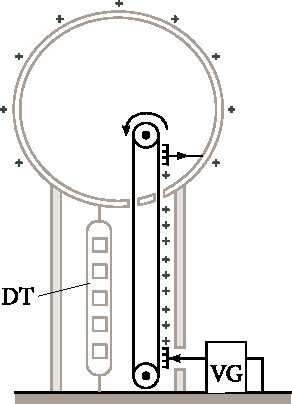
\includegraphics[scale=1]{figures/ch_10/fig_10_14.pdf}
		\caption[]{}
		\label{fig:10_14}
	\end{center}
	\vspace{-0.8cm}
\end{figure}

\textbf{The Van De Graaff Generator}. In 1929, R. van de Graaff proposed an electrostatic generator based on the fact that surplus charges take up a position on the external surface of a conductor.
A schematic view of the generator is shown in \fig{10_14}.
A hollow metal sphere called a conductor is mounted
on an insulating column.
An endless moving belt of silk or rubberized fabric mounted on shafts is introduced into the sphere.
A comb of sharp points is installed at the base of the column near the belt.
The charge produced by a voltage generator (VG) for several scores of kilovolts flows onto the belt from
the comb points.
The conductor contains a second comb onto whose points the charge flows from the belt.
This comb is connected \fig{10_14} to the conductor so that the charge taken off the belt immediately passes over to its external surface.
As charges accumulate on the conductor, its potential grows until the charge that leaks away becomes equal to the newly supplied charge.
The leakage is mainly due to ionization of the gas near the surface of the conductor.
The resulting passage of a current through the gas is called a corona discharge (see \sect{12_8}).
The surface of the conductor is carefully polished to reduce the corona discharge.

The potential up to which the conductor can be discharged is limited by the circumstance that at a field strength of about \SI{3}{\kilo\volt\per\metre}
(\SI{30}{\kilo\volt\per\centi\metre}) a discharge appears in the air at atmospheric pressure.
For a sphere, $E=\varphi/r$.
Therefore, to obtain higher potential differences, the size of the conductor has to be increased (up to \SI{10}{\metre} in diameter).
The maximum potential difference that can be obtained in practice with the aid of a van de Graaff generator is about \SI{10}{\mega\volt} (\SI{e7}{\volt}).

Particles are accelerated in a discharge tube (DT) to whose electrodes the potential difference obtained in the generator is applied.
A van de Graaff generator is sometimes designed in the form of two identical columns near each other whose conductors are charged oppositely.
In this case, the discharge tube is connected between the conductors.

It must be noted that the generator belt, conductor, discharge tube, and the earth form a closed direct current circuit.
Inside the tube, the charges move under the action of the electrostatic field.
Charges are carried to the conductor from the earth by extraneous forces whose part is played by the mechanical forces bringing the generator belt into motion.

\begin{figure}[t]
	\begin{center}
		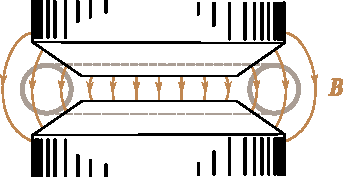
\includegraphics[scale=1]{figures/ch_10/fig_10_15.pdf}
		\caption[]{}
		\label{fig:10_15}
	\end{center}
	\vspace{-0.8cm}
\end{figure}

\textbf{Betatron.} This is the name given to an induction accelerator of electrons using a vortex electric field.
It consists of a toroidal evacuated chamber (a doughnut) placed between the poles of an electromagnet of a special shape (\fig{10_15}).
The winding of the magnet is supplied with alternating current having a frequency of about \SI{100}{\hertz}.
The varying magnetic field produced performs two functions: first, it sets up a vortex electric field accelerating the electrons, and, second, it retains the electrons in an orbit coinciding with the axis of the doughnut.

To keep an electron in an orbit of constant radius, the magnetic induction of the field must be increased as its velocity grows [according to \eqn{10_2}, the radius of the orbit is proportional to $v/B$].
Consequently, only the second and fourth quarters of the current period can be used for acceleration because at their beginning the current in the magnet winding is zero.
A betatron thus operates in pulse conditions.
At the beginning of the pulse, an electron gun feeds a beam of electrons into the doughnut.
The beam is caught up by the vortex electric field and begins to travel in a circular orbit with a constantly growing velocity.
During the growth of the magnetic field (about \SI{e-3}{\second}), the electrons are able to complete up to a million revolutions and acquire an energy that may reach several hundred \si{\mega\electronvolt}.
With such an energy, the speed of the electrons almost equals the speed of light $c$.

For an electron being accelerated to travel in a circular orbit of radius $r_0$, a simple relation, which we shall now proceed to derive, must be observed between the magnetic induction of the field in the orbit and inside it.
The vortex electric field is directed along a tangent to the orbit along which the electron is travelling.
Hence, the circulation of the vector $\vec{E}$ along this orbit is $2\pi r_0E$.
At the same time according to \eqn{9_19}, the circulation of the vector $\vec{E}$ is $-(\diffin{\Phi}{t})$, where $\Phi$ is the magnetic flux through the surface enclosed by the orbit.
The minus sign indicates the direction of $\vec{E}$.
We shall be interested only in the magnitude of the field strength, therefore, we shall omit the minus sign.
Equating the two expressions for the circulation, we find that
\begin{equation*}
    E = \frac{1}{2\pi r_0} \diff{\Phi}{t}.
\end{equation*}

\noindent
The magnetic field is perpendicular to the plane of the orbit.
We can, therefore, assume that $\Phi=\pi r^2_0\average{B}$, where $\average{B}$ is the average
value of the magnetic induction over the area of the orbit.
Hence,
\begin{equation}\label{eq:10_30}
    E = \frac{1}{2\pi r_0} \diff{}{t} \parenthesis{ \pi r^2_0 \average{B}} = \frac{r_0}{2} \diff{}{t} \average{B}.
\end{equation}

Let us write the relativistic equation of motion of an electron in orbit:
\begin{equation}\label{eq:10_31}
    \diff{}{t}\bracket{ \frac{m \vec{v}}{\sqrt{1-\parenthesis{v^2/c^2}}} } = e \vec{E} + e \vec{v} \times \ab{\vec{B}}{orb}
\end{equation}

\noindent
($\ab{\vec{B}}{orb}$ is the magnetic induction of the field in the orbit).

The velocity of an electron moving along a circle of radius $r_0$ can be written in the form $\vec{v}=\omega r_0 \hatvec{\tau}$, where $\omega$ is the angular velocity of the electron, and $\hatvec{\tau}$ is the unit vector of a tangent to the orbit.
The vector $\vec{E}$ can be represented in the form
\begin{equation*}
    \vec{E} = E \hatvec{\tau} = \frac{r_0}{2} \diff{}{t} \average{B} \hatvec{\tau}
\end{equation*}

\noindent
[see \eqn{10_30}].
Finally, the product $\vecprod{v}{B}$ can be written in the form $vB\hatvec{n}=\omega r_0 B\hatvec{n}$, where $\hatvec{n}$ is a unit vector of a normal to the orbit.
In view of what has been said above, let us write \eqn{10_31} as follows:
\begin{equation}\label{eq:10_32}
    \diff{}{t}\bracket{ \frac{\omega r_0 \hatvec{\tau}}{\sqrt{1 - \parenthesis{\omega^2r_0^2/c^2}}} } = \frac{er_0}{2} \diff{}{t} \average{B} \hatvec{\tau} + e\omega r_0 \ab{B}{orb} \hatvec{n}.
\end{equation}

The time derivative of the unit vector $\hatvec{\tau}$ is $\hatvec{\tau}=\omega\hatvec{n}$ [see Eq. (1.56) of Vol. I; the angular velocity of rotation of the unit vector $\hatvec{\tau}$ coincides with the angular velocity of an electron].
Consequently, performing differentiation in the left-hand side of \eqn{10_32}, we arrive at the equation
\begin{equation*}
    \diff{}{t}\bracket{ \frac{\omega r_0}{\sqrt{1 - \parenthesis{\omega^2r_0^2/c^2}}} } \hatvec{\tau} + \bracket{ \frac{\omega r_0}{\sqrt{1 - \parenthesis{\omega^2r_0^2/c^2}}} } \omega \hatvec{n} = \frac{e r_0}{2} \diff{}{t} \average{B} \hatvec{\tau} + e \omega r_0 \ab{B}{orb} \hatvec{n}.
\end{equation*}

\noindent
Equating the factors of similar unit vectors in the left-hand and righthand sides of the equation, we get
\begin{align}
    \diff{}{t}\bracket{ \frac{\omega r_0}{\sqrt{1 - \parenthesis{\omega^2r_0^2/c^2}}} } &= \frac{e r_0}{2} \diff{}{t} \average{B}, \label{eq:10_33}\\
    \frac{\omega r_0}{\sqrt{1 - \parenthesis{\omega^2r_0^2/c^2}}} &= er_0 \ab{B}{orb}. \label{eq:10_34}
\end{align}

\noindent
It follows from \eqn{10_33} that
\begin{equation}\label{eq:10_35}
    \frac{\omega r_0}{\sqrt{1 - \parenthesis{\omega^2r_0^2/c^2}}} = \frac{e r_0}{2} \average{B}
\end{equation}

\noindent
($\omega$ and $\average{B}$ at the beginning of a pulse equal zero).

A comparison of \eqns{10_34}{10_35} yields:
\begin{equation*}
    \ab{B}{orb} = \frac{1}{2} \average{B}.
\end{equation*}

\noindent
Thus, for an electron to travel constantly in a circular orbit, the magnetic induction in the orbit must be half of the average value of the magnetic induction inside the orbit.
This is achieved by making the pole shoes in the form of truncated cones (see \fig{10_15}).

At the end of an acceleration cycle, an additional magnetic field is switched on that deflects the accelerated electrons from their stationary orbit and directs them onto a special target inside the doughnut.
Upon striking the target, the electrons emit hard electromagnetic radiation (gamma rays, X-rays).

Betatrons are mainly used in nuclear investigations. Small accelerators for an energy up to \SI{50}{\mega\electronvolt} have found use in industry as sources of very hard X-rays employed for flaw detection in massive articles.

\textbf{Cyclotron.} The accelerator bearing this name is based on the period of revolution of a charged particle in a homogeneous magnetic field being independent of its velocity [see \eqn{10_3}].
This apparatus consists of two electrodes in the form of halves of a low round box (\fig{10_16}\footnote{This figure was taken from \texttt{https://commons.wikimedia.org/wiki/File:Zyclotron.svg}.}) called dees.
The latter are confined in an evacuated housing placed between the poles of a large electromagnet.
The field produced by the magnet is homogeneous and perpendicular to the plane of the dees.
The dees are supplied with an alternating voltage produced by a high-frequency generator.

\begin{figure}[t]
	\begin{center}
		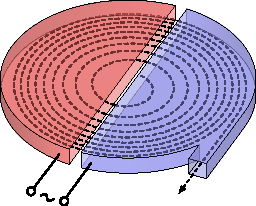
\includegraphics[scale=1]{figures/ch_10/fig_10_16.pdf}
		\caption[]{}
		\label{fig:10_16}
	\end{center}
	\vspace{-0.8cm}
\end{figure}

Let us introduce a charged particle into the slit between the dees at the moment when the voltage reaches its maximum value.
The particle will be caught up by the electric field and pulled into one of the dees.
The space inside the dee is equipotential, therefore, the particle in it will be under the action of only a magnetic field.
In this case, the particle travels along a circle whose radius is proportional to the velocity of the particle [see \eqn{10_2}].
Let us choose the frequency of the change in the voltage between the dees so that by the moment when the particle, after covering half of the circle, approaches the slit between the dees, the potential difference between them will change its sign and reach its amplitude value.
The particle will now be accelerated again and fly into the second dee with an energy double that with which it travelled in the first dee.
Having a greater velocity, the particle will travel in the second dee along a circle of a greater radius ($R$ is proportional to $v$), but the time during which it covers half the circle remains the same as previously.
Therefore, by the moment when the particle flies into the slit between the dees, the voltage between them will again change its sign and take on the amplitude value.

Thus, the particle travels along a curve close to a spiral, and each time it passes through the slit between the dees it receives an additional portion of energy equal to $e'\ab{U}{m}$ ($e'$ is the charge of the particle, and $\ab{U}{m}$ is the amplitude of the voltage produced by the generator).
Having a source of alternating voltage of a comparatively small value ($\ab{U}{m}$ is about \SI{e5}{\volt}) at our disposal, we can use a cyclotron to accelerate protons up to energies of about \SI{25}{\mega\electronvolt}.
At higher energies, the dependence of the mass of the protons on the velocity begins to tell---the period of revolution increases [according to \eqn{10_3} it is proportional to $m$], and the synchronism between the motion of the particles and the changes in the accelerating field is violated.

To prevent this violation of synchronism and to obtain particles having higher energies, either the frequency of the voltage fed to the dees or the magnetic field induction is made to vary.
An apparatus in which in the course of accelerating each portion of particles the frequency of the accelerating voltage is diminished as required is called a \textbf{phasotron} (or a \textbf{synchrocyclotron}).
An accelerator in which the frequency remains constant, while the magnetic field induction is changed so that the ratio $m/B$ remains constant is called a \textbf{synchrotron} (equipment of this type is used only to accelerate electrons).

In the accelerator called a \textbf{synchrophasotron} or a proton synchrotron, both the frequency of the accelerating voltage and the magnetic field induction are changed.
The particles being accelerated travel in this machine along a circular path instead of a spiral.
An increase in the velocity and mass of the particles is attended by a growth in the magnetic field induction so that the radius determined by \eqn{10_2} remains constant.
The period of revolution of the particles changes both owing to the growth in their mass and to the growth in $B$.
For the accelerating voltage to be synchronous with the motion of the particles, the frequency of this voltage is made to change according to the relevant law.
A synchrophasotron has no dees, and the particles are accelerated on separate sections of the path by the electric field produced by the varying frequency voltage generator.

The most powerful accelerator at present (in 1979)---a proton synchrotron---was started in 1974 at the Fermi National Accelerator Laboratory at Batavia, Illinois, in the USA.
It accelerates protons up to an energy of \SI{400}{\giga\electronvolt} (\SI{4e11}{\electronvolt}).
The speed of protons having such an energy differs from that of light in a vacuum by less than $0.0003\%$ ($v = 0.9999972c$).
